\documentclass[aspectratio=169]{beamer}
\usepackage{graphicx}
\usepackage{tikz}
\usepackage{amsmath}
\usepackage{booktabs}
\usetikzlibrary{arrows.meta,positioning,fit,calc,decorations.pathmorphing,backgrounds}

% ---- theme ----
\usetheme{default}
\usecolortheme{default}
\setbeamertemplate{navigation symbols}{}
\setbeamertemplate{footline}[frame number]
\definecolor{accent}{HTML}{2A6F97}
\definecolor{accent2}{HTML}{C1440E}
\definecolor{good}{HTML}{2D6A4F}
\definecolor{ink}{HTML}{22303C}
\setbeamercolor{frametitle}{fg=accent}
\setbeamercolor{title}{fg=accent}
\setbeamercolor{structure}{fg=accent}
\setbeamercolor{block title}{bg=accent!12,fg=accent}
\setbeamercolor{block body}{bg=accent!5}
\setbeamerfont{frametitle}{size=\Large,series=\bfseries}
\setbeamertemplate{itemize item}{\color{accent}\textbullet}
\setbeamertemplate{itemize subitem}{\color{accent}--}

% ---- takeaway: blue background block ----
\setbeamercolor{takeaway}{bg=accent!15,fg=ink}
\newcommand{\take}[1]{%
  \vspace{0.15cm}%
  \begin{beamercolorbox}[wd=\textwidth,sep=5pt,rounded=true]{takeaway}%
    \raggedright\footnotesize#1%
  \end{beamercolorbox}%
}

\title{\textbf{Teaching a Super-Resolution Model to Build Subhalos}}
\subtitle{Direct fine-tuning of SR2 on the particles that matter}
\author{}
\date{}

\begin{document}

% =====================================================
\begin{frame}
\titlepage
\end{frame}

% =====================================================
\section{Background}

% ----- What is a DM simulation / why we need one -----
\begin{frame}{Dark-matter simulations: what they are, why we need them}
\small
We cannot rerun the universe. A simulation is our only \textbf{forward model}: assume a cosmology and
a dark-matter model, let gravity pull a huge cloud of \textbf{particles} together into \textbf{halos},
and predict what a survey should see.

\vspace{0.15cm}
\centering
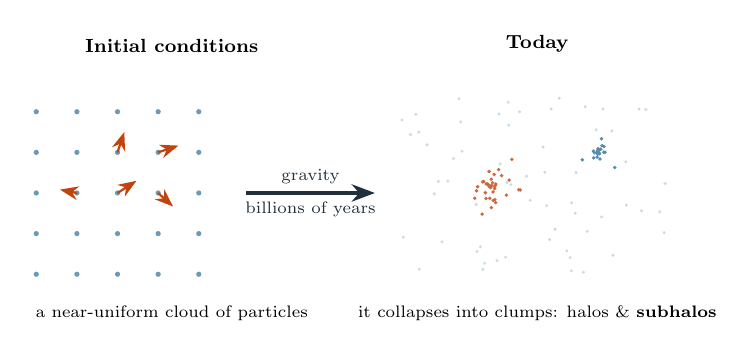
\begin{tikzpicture}[scale=0.86,every node/.style={transform shape}]
% initial conditions: near-uniform grid + small perturbations
\node[above] at (2,3.15) {\footnotesize\textbf{Initial conditions}};
\node[below] at (2,-0.35) {\scriptsize a near-uniform cloud of particles};
\foreach \x in {0,...,4}{\foreach \y in {0,...,4}{
  \fill[accent!70] (\x*0.6,\y*0.6) circle (1.1pt);
}}
% a few perturbation arrows
\foreach \x/\y/\dx/\dy in {2/2/0.28/0.18, 3/2/0.22/-0.2, 2/3/0.1/0.3, 3/3/0.3/0.1, 1/2/-0.25/0.05}{
  \draw[->,accent2,thick,>=Stealth] (\x*0.6,\y*0.6) -- ++(\dx,\dy);
}
\node[align=center,accent2] at (2,-0.05) {};

% arrow between panels
\draw[->,>=Stealth,line width=1.2pt,ink] (3.1,1.2) -- node[above,font=\scriptsize]{gravity} node[below,font=\scriptsize]{billions of years} (5.0,1.2);

% today: clustered points
\begin{scope}[xshift=5.4cm]
\node[above] at (2,3.15) {\footnotesize\textbf{Today}};
\node[below] at (2,-0.35) {\scriptsize it collapses into clumps: halos \& \textbf{subhalos}};
% background scatter
\foreach \i in {1,...,60}{
  \pgfmathsetmacro\rx{4*rnd}\pgfmathsetmacro\ry{2.6*rnd}
  \fill[accent!25] (\rx,\ry) circle (0.7pt);
}
% a clump
\foreach \i in {1,...,40}{
  \pgfmathsetmacro\a{360*rnd}\pgfmathsetmacro\r{0.55*rnd*rnd}
  \fill[accent2!80] ({1.3+\r*cos(\a)},{1.3+\r*sin(\a)}) circle (0.8pt);
}
\foreach \i in {1,...,22}{
  \pgfmathsetmacro\a{360*rnd}\pgfmathsetmacro\r{0.4*rnd*rnd}
  \fill[accent!80] ({2.9+\r*cos(\a)},{1.8+\r*sin(\a)}) circle (0.8pt);
}
\end{scope}
\end{tikzpicture}

\vspace{0.15cm}
\raggedright\footnotesize
\textbf{Subhalos are the payoff:} each one hosts a galaxy, so their \emph{abundance} is what we match
to observed satellite counts --- and it is where cold, warm and self-interacting DM actually differ.

\take{Getting the large-scale field right is not enough --- \textbf{subhalo abundance is the number
that carries the science.}}
\end{frame}


% ----- Why SR -----
\begin{frame}{Why super-resolution?}
\small
High-resolution simulations resolve small structure --- but the cost explodes with particle count.
Super-resolution learns to \textbf{upsample a cheap low-res run} into something that looks high-res.

\vspace{0.2cm}
\centering
\includegraphics[width=0.72\textwidth]{figures/cost.png}

\vspace{0.1cm}
\take{Run the expensive HR simulation \emph{once} to train; then produce HR-quality fields from
LR inputs for a fraction of the cost. That is the promise --- if the small structure comes out right.}
\end{frame}

% =====================================================
\section{SR2}

% ----- What is SR2 -----
\begin{frame}{SR2: a SOTA baseline}
\small
A \textbf{GAN} super-resolution model (Ni et al.). A \textbf{generator} upsamples the Lagrangian
LR field \textit{\scriptsize(Lagrangian: a fixed grid of particles, each carrying a displacement and a velocity)};
the same particles, displaced onto a mesh, give the \textbf{Eulerian} density field
\textit{\scriptsize(Eulerian: mass counted on a fixed grid in space --- what a survey sees)}.
A single \textbf{critic} judges realism, and it sees \emph{both} representations.

\vspace{0.35cm}
\centering
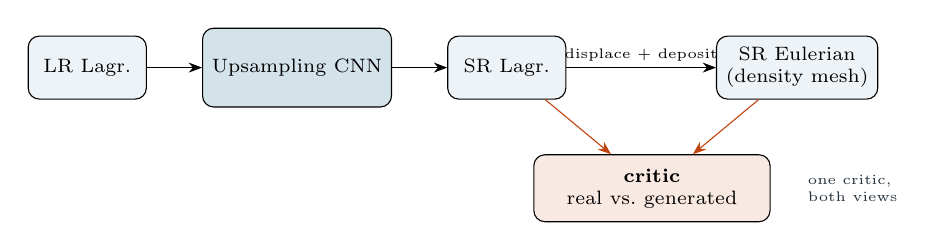
\begin{tikzpicture}[node distance=0.55cm and 0.7cm,every node/.style={font=\scriptsize}]
\node[draw,rounded corners,fill=accent!8,minimum height=0.8cm,minimum width=1.5cm] (lr) {LR Lagr.};
\node[draw,rounded corners,fill=accent!20,align=center,right=of lr,minimum height=1.0cm,minimum width=1.9cm] (g) {Upsampling CNN};
\node[draw,rounded corners,fill=accent!8,right=of g,minimum height=0.8cm,minimum width=1.5cm] (sr) {SR Lagr.};
\node[draw,rounded corners,fill=accent!8,align=center,right=1.9cm of sr,minimum height=0.8cm,minimum width=2.0cm] (eu) {SR Eulerian\\(density mesh)};
\draw[->,>=Stealth] (lr)--(g);
\draw[->,>=Stealth] (g)--(sr);
\draw[->,>=Stealth] (sr)--node[above,font=\tiny,inner sep=2pt]{displace + deposit}(eu);
\coordinate (mid) at ($(sr)!0.5!(eu)$);
\node[draw,rounded corners,fill=accent2!12,align=center,below=1.1cm of mid,
      minimum height=0.85cm,minimum width=3.0cm] (c) {\textbf{critic}\\real vs.\ generated};
\draw[->,>=Stealth,accent2] (sr) -- (c);
\draw[->,>=Stealth,accent2] (eu) -- (c);
\node[ink,font=\tiny,align=left,right=0.35cm of c] {one critic,\\both views};
\end{tikzpicture}

\vspace{0.35cm}
\begin{block}{Strength: SR2 reproduces HR's power spectrum at every scale}
\centering\footnotesize
\begin{tabular}{l c c c c}
\toprule
band $k$ $[h/\mathrm{Mpc}]$ & $0.08$--$1$ & $1$--$4$ & $4$--$16$ & $16$--$32$ \\
\midrule
SR2 $P(k)$ vs.\ HR (band mean) & $+0.8\%$ & $+2.7\%$ & $-0.1\%$ & $+0.4\%$ \\
worst single $k$-bin in band & $1.3\%$ & $4.5\%$ & $3.0\%$ & $1.7\%$ \\
\bottomrule
\end{tabular}

\vspace{0.12cm}
\raggedright\scriptsize\textcolor{ink}{Density $P(k)$ on held-out set9, $1024^3$ mesh. The
statistical distribution of structure is right to a few percent, over nearly three decades of scale.}
\end{block}
\end{frame}

% ----- Weakness: subhalo occupance + bell curves -----
\begin{frame}{SR2's weakness: the small structure is too soft}
\small
Inside big halos live smaller bound clumps --- \textbf{subhalos}. SR2 under-produces them.
A subhalo is a \textbf{sharp density spike}; SR2 makes a \emph{blurred} one.

\vspace{0.1cm}
\begin{columns}[T]
\begin{column}{0.56\textwidth}
\centering
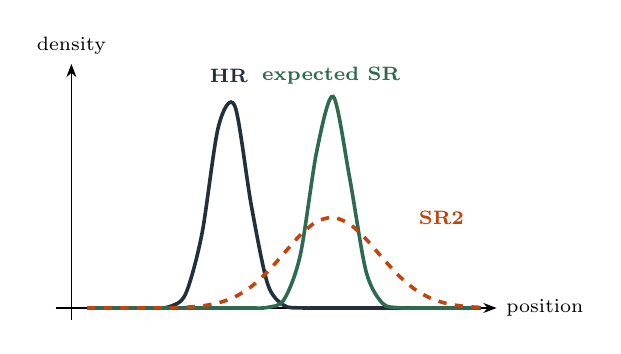
\begin{tikzpicture}[scale=1.0]
\draw[->,>=Stealth] (-0.2,0)--(5.4,0) node[right,font=\scriptsize]{position};
\draw[->,>=Stealth] (0,-0.15)--(0,3.1) node[above,font=\scriptsize]{density};
% HR sharp bell at x=2
\draw[domain=0.2:5.2,smooth,variable=\x,ink,line width=1.3pt]
  plot ({\x},{2.7*exp(-9*(\x-2)*(\x-2))});
% expected SR sharp bell displaced at x=3.3
\draw[domain=0.2:5.2,smooth,variable=\x,good,line width=1.3pt]
  plot ({\x},{2.7*exp(-9*(\x-3.3)*(\x-3.3))});
% SR2 broad low bell at x=3.3
\draw[domain=0.2:5.2,smooth,variable=\x,accent2,line width=1.3pt,dashed]
  plot ({\x},{1.15*exp(-1.4*(\x-3.3)*(\x-3.3))});
\node[ink,font=\scriptsize\bfseries] at (2,2.95) {HR};
\node[good,font=\scriptsize\bfseries] at (3.3,2.95) {expected SR};
\node[accent2,font=\scriptsize\bfseries,align=center] at (4.7,1.15) {SR2};
\end{tikzpicture}

\vspace{0.05cm}
{\scriptsize The LR field can't fix the \emph{position}, so a displaced-but-sharp
spike (green) is an acceptable answer. A \emph{soft} spike (red) is not.}
\end{column}
\begin{column}{0.42\textwidth}
\centering
\vspace{0.3cm}
\begin{block}{The occupation gap}
\centering
\begin{tabular}{lc}
\toprule
subhalos per host & vs.\ HR \\
\midrule
HR (truth) & 100\% \\
SR2 subhalos & \alert{$\sim$18\%} \\
\bottomrule
\end{tabular}
\end{block}
\footnotesize
Measured over \textbf{all 7138 held-out hosts} ($\sim$5\% in the richest clusters).
Positions are unrecoverable from LR --- so we do \textbf{not} demand the right location;
we demand a spike \textbf{as sharp and as bound} as HR's.
\end{column}
\end{columns}
\end{frame}

% ----- Why hard -----
\begin{frame}{Why is this hard?}
\small
Two facts about a subhalo pull the objective in opposite directions.

\vspace{0.1cm}
\begin{columns}[T]
\begin{column}{0.49\textwidth}
\begin{block}{1. What the object \emph{is}: a correlation}
A subhalo is not a density value --- it is a \textbf{highly correlated set of particles},
gathered around a common centre and gravitationally \textbf{bound}.

\vspace{0.12cm}
\textcolor{accent2}{\textbf{Concretely}}, the clump must \textbf{balance spatial density
against velocity dispersion}:
\begin{itemize}
  \item dense enough --- and \emph{cold} enough --- to be \textbf{self-bound}: a halo at all;
  \item and \textbf{denser than its host background}, or the halo finder never separates it
        from the host.
\end{itemize}

\vspace{0.1cm}
It lives in the \textbf{joint} 6-D configuration of $\sim$100 particles at once ---
no per-voxel density target can express it.
\end{block}
\end{column}

\begin{column}{0.49\textwidth}
\begin{block}{2. What the object \emph{weighs}: almost nothing}
\centering
\begin{tabular}{lr}
\toprule
HR, held-out box (set9) & \\
\midrule
particles in the box & 134{,}217{,}728 \\
in subhalos inside hosts & \alert{4.9\%} \\
median subhalo & \alert{107 particles} \\
\bottomrule
\end{tabular}

\vspace{0.15cm}
\raggedright
And the aggregate the critic sees is \textbf{already right without them}: baseline SR2
matches HR's density power spectrum to \textbf{within 3\%} at \emph{every} resolved scale
($k=1$--$32\,h\,$Mpc$^{-1}$) --- while holding \alert{18\%} of the subhalos.
\end{block}
\end{column}
\end{columns}

\take{\textbf{The conflict:} what \emph{defines} the object is not in the loss, and what
\emph{is} in the loss is already satisfied. A global objective sits at its optimum with the
substructure absent --- so the generator takes the cheap, large-scale solution and
\textbf{oversmooths} the 5\% that matters.}
\end{frame}

% =====================================================
\section{Method}

\begin{frame}{Method: fine-tune the generator, on the right particles}
\small
We \textbf{directly fine-tune SR2's generator alone} (critics frozen). The key move: we know
\emph{which} particles form each HR subhalo (shared Lagrangian ids), so we \textbf{mask the loss to
exactly those particles} --- only they receive gradient.

\vspace{0.15cm}
The loss is a sum of terms, \textbf{each normalised to HR's own value} on the same particle set
(so it never asks for more than HR has). Every term but the bound term is on:

\vspace{0.1cm}
\centering
\begin{tabular}{l l}
\toprule
Term & Why it is needed \\
\midrule
\textbf{virial} $2T/|W|$ & forces the density--dispersion balance (bound, not just dense) \\
\textbf{d6} (6-D compactness) & tight in position \emph{and} velocity vs.\ a \emph{local} background $\Rightarrow$ stands out as a subhalo \\
\textbf{$r_{\mathrm{rms}}$} & fixes the physical \emph{size} of the clump (breaks a size/velocity degeneracy) \\
\textbf{$\sigma_v$} & fixes the \emph{velocity dispersion} (the other half of that degeneracy) \\
\textbf{centre} & pins \emph{where} the object forms, so the mass gathers to one place \\
\bottomrule
\end{tabular}

\vspace{0.2cm}
\footnotesize\textcolor{ink}{Hinged/two-sided so an over-collapsed clump is penalised as much as a diffuse one.
The \emph{bound} term itself is left out here.}
\end{frame}

% =====================================================
\section{Results}

\begin{frame}{Result 1: 92\% subhalo recovery v.s. baseline's 18\%}
\small

\vspace{0.15cm}
\centering
\includegraphics[width=0.98\textwidth]{figures/fig1_zoom_rvir.png}

\vspace{0.1cm}
\centering
\begin{tabular}{l c c}
\toprule
Subhalos in $R_{\mathrm{vir}}$, all 7138 hosts & total (vs.\ HR) & mean per host \\
\midrule
HR (truth) & 7539 \quad(100\%) & 1.06 \\
Baseline SR2 & \alert{1345 \quad(18\%)} & 0.19 \\
\textbf{Tuned (ours)} & \textbf{\textcolor{good}{6964 \quad(92\%)}} & \textbf{\textcolor{good}{0.98}} \\
\bottomrule
\end{tabular}
\end{frame}

\begin{frame}{Result 2: and they are the \emph{right} subhalos}
\small
Not just the right number --- the right \textbf{mass distribution}. Subhalo counts binned by
Rockstar bound-particle count, pooled over the same 7138 held-out hosts.

\vspace{0.1cm}
\centering
\includegraphics[width=0.65\textwidth]{figures/sub_mass_function_log.png}

\vspace{0.05cm}
\take{The tuned model (red) tracks HR (black) in \emph{every} mass bin --- 84\% of HR at
50--100 particles up to 97--108\% at the massive end --- where baseline SR2 (grey) is short by
$5$--$10\times$ across the whole small-mass range. The recovered objects have HR's mass function,
not an arbitrary pile of clumps.}
\end{frame}

\begin{frame}{Result 3: small-scale power --- a slight overshoot}
\small
\begin{itemize}
  \item Large scales are untouched --- under 1\% for $k<1\,h/$Mpc. The excess is a smooth
        $\sim$\alert{35\%} bump peaking near $k\approx12\,h/$Mpc, closing again by the
        mesh Nyquist.
\end{itemize}

\vspace{0.05cm}
\centering
\includegraphics[height=0.8\textheight]{figures/density_power.png}

\end{frame}

% ----- The one gap: radial distribution -----
\begin{frame}{The one gap: our subhalos sit too close to the centre}
\small
We recover the right \emph{number} and \emph{masses} of subhalos --- but not yet the right
\textbf{radial distribution}. Ours pile up near the host centre; HR's fill the halo and extend
past $R_{\mathrm{vir}}$.

\vspace{0.15cm}
\centering
\includegraphics[width=0.5\textwidth]{figures/subhalo_radial_dist.png}

%\vspace{0.1cm}
\begin{columns}[c]
\begin{column}{0.5\textwidth}
\centering
\begin{tabular}{l c}
\toprule
median distance & $R / R_{\mathrm{vir}}^{\mathrm{host}}$ \\
\midrule
HR (truth) & 1.13 \\
\textbf{Tuned (ours)} & \alert{0.35} \\
\bottomrule
\end{tabular}
\end{column}
\begin{column}{0.48\textwidth}
\footnotesize
The masked, host-centred loss gathers mass toward the centre it is given --- so the clumps form,
but too centrally concentrated. Spreading them to HR's radial profile is the natural next target.
\end{column}
\end{columns}
\end{frame}


\begin{frame}
\centering
\vspace{1.2cm}
{\Large\textbf{\textcolor{accent}{Thank you}}}\\[0.4cm]
\normalsize Questions?
\end{frame}

\end{document}
